\section{Adaptação do \textit{client-side prediction} no contexto musical \textit{online}}

Propomos, então, uma variação da implementação de Bernier \cite{client-side-prediction} de previsão no lado do cliente, para sua aplicação no contexto musical (\figref{fig:rollback_music_diagram}). Similarmente à técnica original, janelas de áudios são previstas baseando-se nas entradas anteriores. Entretanto, nenhuma correção é realizada em casos de erro, mantendo a linearidade da música.

\begin{figure}[htbp]
\centering
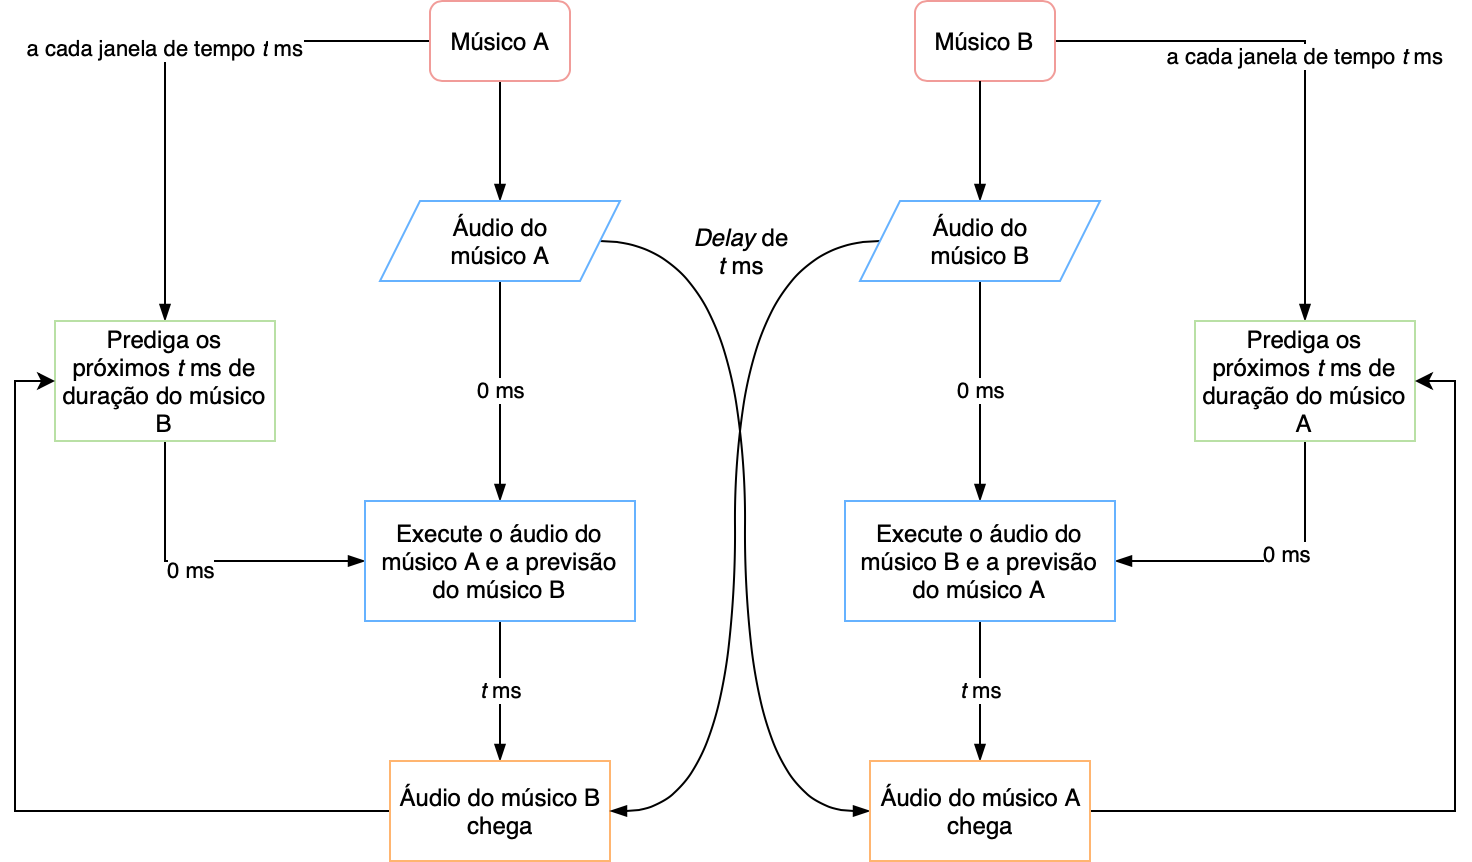
\includegraphics[width=1\textwidth]{images/rollback-music.png}
\caption{Diagrama demonstrando a adaptação do algoritmo de previsão no lado do cliente aplicado para ambiente colaborativo musical \textit{online}. Na imagem, $t$ representa a duração da janela de previsão, medido em milissegundos.}
\label{fig:rollback_music_diagram}
\end{figure}

Em Bernier, a janela de tempo de cada conjunto de previsões é definida de acordo com o FPS do jogo e a velocidade de conexão entre os participantes. Para adaptação musical, além do tempo de ida e volta dos pacotes entre os participantes (denominado \textit{ping}), propomos a utilização de outros parâmetros para a decisão dessa janela, como o BPM (batimentos por minuto) da música tocada junto à informação dos compassos musicais e também, por simplicidade, valores múltiplos de 1 segundo. A escolha dessa janela é fundamental - durações muito longas possuem muita informação, porém, são mais difíceis de processar e mais suposições terão que ser realizadas na previsão; e o inverso ocorre para janelas muito curtas.

Propomos, portanto, dois modelos preditivos para música, explorados em dois ciclos de pesquisa. No \chapref{chap:lstm}, no primeiro ciclo, utilizamos a arquitetura de aprendizagem de máquina em camadas LSTM (\textit{Long Short-Term Memory)} \cite{lstm} para gerar sequências de sinais digitais, baseando-se nas entradas anteriores. Já no \chapref{chap:dtw}, no segundo ciclo, usamos o algoritmo DTW (\textit{Dynamic Time Warping}) \cite{dtw} para identificar janelas semelhantes em uma base de dados e, a partir dessa informação, reproduzir a próxima janela de áudio, também armazenada na mesma base de dados.

É válido mencionar que, no entanto, pela natureza imprevisível das improvisações musicais, esse caso de uso não deve ser bem aplicado em nossa solução proposta. Porém, para bases e sequências de acordes, onde é mais fácil prever as próximas entradas, o uso de nossa solução é melhor adequado.
